%template1.tex
%The following LaTeX source file represents the simplest kind of slide presentation; no overlays, no included graphics. Substitute your favorite style for ``pascal''. To create the PDF file template1.pdf, (1) be sure to use the prosper class, then (2) execute the command latex template1.tex, and (3) the command dvipdf template1.dvi.

%%%%%%%%%%%%%%%%%%%%%%%%%%%%%%% template1.tex %%%%%%%%%%%%%%%%%%%%%%%%%%%%%%%%%%%
\documentclass[a4paper,blends,pdf,colorBG,slideColor]{prosper}
% definitions for slides for CSC544
% Lutz Hamel, (c) 2007

\hypersetup{pdfpagemode=FullScreen}

\usepackage{amssymb}
\usepackage{latexsym}
\usepackage{amsmath}
%\usepackage[usenames]{color}
\usepackage{xypic}


\newcommand{\term}[1]{\ensuremath{\mbox{\bf #1}}}
\newcommand{\nonterm}[1]{\ensuremath{\mbox{#1}}}
\newcommand{\ifstmt}[3]{\ensuremath{{\bf if}\; {#1}\;{\bf then}\;{#2}\;{\bf else}\;{#3}\;\term{end}}}
\newcommand{\whilestmt}[2]{\ensuremath{{\bf while}\; {#1}\;{\bf do}\;{#2}\; \term{end}}}
\newcommand{\funcstmt}[3]{\ensuremath{{\bf fun}\; {#1}\; {\bf is}\; {#2} \; {\bf return}\; {#3}}}
\newcommand{\syntaxset}[1]{\ensuremath{\mbox{\bf #1}}}
\newcommand{\orbar}{\;|\;}
\newcommand{\bs}[1]{\begin{slide}{#1}\ptsize{8}}
\newcommand{\es}{\end{slide}}
\newcommand{\co}{\,\colon\;}
\newcommand{\pair}[2]{\ensuremath{\langle {#1}, {#2} \rangle}}
\newcommand{\encode}[1]{\ensuremath{\langle {#1} \rangle}}
\newcommand{\mytab}{\makebox[.15in]{}}
%\newcommand{\abs}[1]{{\mid{#1}\mid}}
\newcommand{\abs}[1]{{|{#1}|}}
\newcommand{\ol}[1]{\overline{#1}}

\newcommand{\qaccept}{\ensuremath{q_{\mbox{\tiny accept}}}}
\newcommand{\qreject}{\ensuremath{q_{\mbox{\tiny reject}}}}
\newcommand{\accept}{{\em accept}}
\newcommand{\reject}{{\em reject}}

\newcommand{\machine}[1]{
	\begin{quote}
	{#1}
	\end{quote}
	}

\newcommand{\fdef}[1]{
	\begin{center}
	\fbox{
	\begin{minipage}{3.5in}
	{\bf Definition:}
	{#1}
	\end{minipage}
	}
	\end{center}
	}

\newcommand{\ftheorem}[1]{
	\begin{center}
	\fbox{
	\begin{minipage}{3.5in}
	{\bf Theorem:}
	{#1}
	\end{minipage}
	}
	\end{center}
	}

\newcommand{\flemma}[1]{
	\begin{center}
	\fbox{
	\begin{minipage}{3.5in}
	{\bf Lemma:}
	{#1}
	\end{minipage}
	}
	\end{center}
	}


\newcommand{\fframe}[1]{
	\begin{center}
	\fbox{
	\begin{minipage}{3.5in}
	{#1}
	\end{minipage}
	}
	\end{center}
	}

\newcommand{\nframe}[1]{
	\begin{center}
	\begin{minipage}{3.5in}
	{#1}
	\end{minipage}
	\end{center}
	}

\begin{document}

\bs{$P$ and $NP$}
\fdef{$P$ is the class of languages that are decidable in polynomial time on a deterministic Turing machine,
\[
P = \bigcup_k TIME(n^k), \mbox{ for $k \ge 0$.}
\]}

\fdef{
\[
NP = \bigcup_k NTIME(n^k), \mbox{ for $k \ge 0$}.
\]}

{\bf Observation:} In order to prove that a language is a member of a particular
complexity class we simply have to demonstrate than an appropriate algorithm
exists.  

We have seen this in the case of the directed path in a graph.
\es

\bs{Properties of $P$ and $NP$}
\fframe{{\bf Theorem:} The complexity class $P$ is closed under complementation.}

{\bf Proof:} Any language $L \in P$ can be decided in deterministic polynomial time.  Let $M$
be such a decider for $L$.  To show that $P$ is closed under complementation we show that
we can construct a deterministic polynomial time decider $M'$ for $\overline{L}$,
\begin{quote}
$M'$ = "On input $w$, where $w$ is a string:
\begin{itemize}
\item[1.] Run $M$ on $w$.
\item[2.] If $M$ accepts, \reject; if $M$ rejects, \accept."
\end{itemize}
\end{quote}
It is easy to see that this machine runs in deterministic polynomial time. $\Box$
\es


\bs{Properties of $P$ and $NP$}
{\small
\fframe{{\bf Theorem:} The complexity class $NP$ is closed under the Kleene-closure.}

{\bf Proof:} Any language $L$ in $NP$ is decided by some nondeterministic polynomial time TM.  Let $M$ be such a decider for $L$.  To show that $NP$ is closed under the Kleene-closure we need to show that
$L^* \in NP$, where \[L^* = \{ w | \mbox{$w = \emptyset$ or $w = w_1 w_2 \ldots w_k$ for $k \ge 1$ and each $w_i \in L$} \}.\]
We construct a nondeterministic polynomial time TM $M'$ that decides $L^*$,
\begin{quote}
$M'$ = "On input $w$, where $w$ is a string:
\begin{itemize}
\item[1.] If $w = \emptyset$, then \accept.
\item[2.] Nondeterministically split $w$ into the strings $w_1 w_2 \ldots w_k$ for $k \ge 1$.
\item[3.] Run $M$ on each string $w_i$.
\item[4.] If $M$ accepts all $w_i$'s, \accept; otherwise, \reject."
\end{itemize}
\end{quote}
By realizing that the number of times the machine $M$ is invoked is bounded by $O(n)$ (each $|w_i| = 1$
with $n = |w|$) and the fact that $M$ is a nondeterministic polynomial time TM, say $O(n^m)$, then the total nondeterministic polynomial runtime is $O(n^{m+1})$ .  Therefore, $L^* \in NP$. $\Box$
}
\es


\bs{Hamiltonian Path}
{\small
A Hamiltonian path in a directed path is a directed path that goes through each node exactly once.  Formally, $HAMPATH = \{ \encode{G,s,t}| G$ is a directed graph
with a Hamiltonian path from $s$ to $t \}$.

No deterministic polynomial time algorithms are know that decide this language.

\fframe{{\bf Theorem:} \[HAMPATH \in NP\]}

{\bf Proof:} We construct an nondeterministic Turing machine that decides $HAMPATH$
in polynomial time.

\begin{quote}
$M$ = "On input $\encode{G,s,t}$:
\begin{itemize}
\item[1.] Nondeterministically generate a permutation of $m$ numbers $p_1,\ldots,p_m$ such that $1 \le p_i \le m$ where $m$ is the 
number of nodes in graph $G$.  
 \item[2.] Check whether $p_1 = s$ and $p_m = t$.
 If either test fails, \reject.
 \item[3.] For each $i$ between $1$ and $m-1$, check wether  $(p_i, p_{i+1})$
 is an edge in $G$. If any are not, \reject.  Otherwise, the generated list
 of numbers represents a Hamiltonian path, \accept."
\end{itemize}
\end{quote}
Analysis. It is easy to see that all the stages run in polynomial time.  $\Box$
}
\es

\bs{Verifiers}
We can define the class $NP$ in an alternative manner using deterministic polynomial time verifiers.

\fdef{A {\bf\em verifier} for a language $A$ is a deterministic TM $V$, where
\[
A = \{ w | \mbox{$V$ accepts $\encode{w,c}$ for some string $c$} \}.
\]}

Here the string $c$ is called a {\bf\em certificate}.

We measure the time of a verifier in terms of the length of $w$, that is, a 
polynomial time verifier run in polynomial time in the length of $w$.

A language is {\bf\em polynomially verifiable} if it has a (deterministic) polynomial time verifier.

\fdef{$NP$ is the class of languages that have (deterministic) polynomial time verifiers.}
\es


\bs{Hamiltonian Path (revisited)}
{\small
\fframe{{\bf Theorem:} \[HAMPATH \in NP\]}

{\bf Proof \#2:}  This time we show that a polynomial time verifier exists for 
a Hamiltonian path.

Let $c$ be a Hamiltonian path $\encode{p_1 \leadsto p_m}$, the we construct
the verifier $V$ as follows:

\begin{quote}
$V$ = "On input $\encode{\encode{G,s,t},c}$:
\begin{itemize}
\item[1.] Verify that $|p_1 \leadsto p_m| = m - 1$.  If not, \reject.
\item[2.] Verify that $p_1 \leadsto p_m$ does not have any repetitions.  If any are found,
\reject.
\item[3.] Check wether $p_1 = s$ and $p_m = t$.  If either fails, \reject.
\item[4.] For each $i$ between $1$ and $m-1$, check wether  $(p_i, p_{i+1})$
 is an edge in $G$. If any are not, \reject. 
\item[5.] All test have passed, \accept."
\end{itemize}
\end{quote}
}
\es

\bs{Deciding vs. Verifying}
{\small
\fframe{{\bf Theorem:} A language is decided by a nondeterministic polynomial time TM  iff it can be verified by a deterministic polynomial time verifier.}

{\bf Proof:} We show that nondeterministic deciders can be constructed from verifiers and vice versa.

(a) For the `$\Rightarrow$' direction: Let $N$ be the nondeterministic TM that decides the language, then we can construct a corresponding verifier $V$ as follows,
\begin{quote}
$V$ = " On input $\encode{w,c}$, where $w$ and $c$ are strings:
\begin{itemize}
\item[1.] Simulate $N$ on $w$ but only follow computations that are described in $c$
(this means $N$ will only have a single branch of computation).
\item[2.] If this branch of computation accepts, \accept; otherwise, \reject."
\end{itemize}
\end{quote}

(b) For the `$\Leftarrow$' direction: Let $V$ be a polynomial time verifier with runtime $n^k$, then we can construct
the corresponding nondeterministic TM $N$,
\begin{quote}
$N$  = "On input $w$ of length $n$:
\begin{itemize}
\item[1.] Nondeterministically generate a string $c$ with $|c| \le n^k$.
\item[2.] Run $V$ on $\encode{w,c}$.
\item[3.] If $V$ accepts, \accept; otherwise, \reject."
\end{itemize}
\end{quote}
}
\es

\bs{Cliques}
{\bf Example:} Clique in a graph.  A clique in an undirected graph is a subgraph wherein every  two nodes  are connected by an edge.  A $k$-clique is a clique that
has $k$ node.
\begin{center}
\includegraphics[height=20mm]{images/5-clique.eps}{A 5-clique.}
\end{center}
Formally, expressed as a language, \[CLIQUE = \{ \encode{G,k}| \mbox{$G$ is an undirected graph with a $k$-clique }\}.\]

\es

\bs{$CLIQUE \in NP$}
{
\fframe{{\bf Theorem:} 
\[
CLIQUE \in NP.
\]}

{\bf Proof \#1:} We construct a nondeterministic polynomial time decider.
\begin{quote}
$N$ = "On input $\encode{G,k}$:
\begin{itemize}
\item[1.] Nondeterministically select a set $Q$ of $k$ nodes where each node is in $G$.
\item[2.] Test whether $G$ contains all edges connecting nodes in $Q$.
\item[3.] If yes, \accept; otherwise, \reject."
\end{itemize}
\end{quote}
Stage 2 runs in $O(n^2)$ with $n = |\encode{G,k}|$.  Therefore, there whole machine
runs in nondeterministic polynomial time.
}
\es

\bs{$CLIQUE \in NP$}
{\bf Proof \#2:} Let $c$ be a $k$-clique on $G$, then construct a verifier,
\begin{quote}
$V$ = "On input $\encode{\encode{G,k},c}$:
\begin{itemize}
\item[1.] Test whether $c$ is a set of $k$ nodes in $G$.
\item[2.] Test whether $G$ contains all edges connecting nodes in $Q$.
\item[3.] If all tests pass, \accept; otherwise, \reject."
\end{itemize}
\end{quote}
Here, stage 1 and 2 run in $O(n^2)$ time, therefore the verifier runs in deterministic
polynomial time.
\es

\bs{$P$ vs $NP$}

Since a TM is considered a special case of an nondeterminisic TM we have,
\[
P \subset NP
\]
It is still an open question whether $P = NP$, since currently the best known 
deterministic algorithms for $NP$ problems use exponential time,
\[
NP \subseteq EXPTIME = \bigcup_k TIME(2^{n^k})
\]
(Remember: to simulate a nondeterministic TM on a TM we need exponential time.)
\es

\bs{$NP$-Completeness}
\fframe{{\bf Definition:} A function $f\co \Sigma^* \rightarrow \Sigma^*$ is a 
{\bf\em polynomial time computable function} if some (deterministic) polynomial time Turing machine $M$, on every input $w$,
halts with just $f(w)$ on its tape.}

\vspace{.2in}

\fframe{{\bf Definition:} Language $A$ is {\bf\em polynomial time mapping reducible}, or simply {\bf \em polynomial time reducible},  to language
$B$, written $A \le_p B$, if  a polynomial time computable function $f\co \Sigma^* \rightarrow \Sigma^*$ exists, where for every $w$,
\[
w \in A \Leftrightarrow f(w) \in B.
\]
The function $f$ is call the {\bf\em polynomial time reduction} from $A$ to $B$.}

\es

\bs{$NP$-Completeness}
\fframe{{\bf Theorem:} If $A \le_p B$ and $B \in P$ , then $A\in P$.}

{\bf Proof:} Let $M$ be a polynomial time decider for $B$ and let $f$ be a polynomial time reduction from $A$ to $B$,
then we can construct a polynomial time decider $N$ for $A$ as follows:

\begin{quote}
$N$ = "On input $w$:
\begin{enumerate}
\item[1.] Compute $f(w)$.
\item[2.] Run $M$ on $f(w)$ and output whatever $M$ outputs."
\end{enumerate}
\end{quote}

Clearly, if $w \in A$ then $f(w) \in B$ since $f$ is a reduction.
It is easy to see that $N$ runs in polynomial time.$\Box$
\es

\bs{$NP$-Completeness}
\fdef{A language $Q$ is {\bf\em NP-complete} if it satisfies two conditions:
\begin{enumerate}
\item $Q \in NP$, and
\item every $Q_i \in NP$ is polynomial time reducible to $Q$.
\end{enumerate}}

\vspace{.5in}

\begin{center}
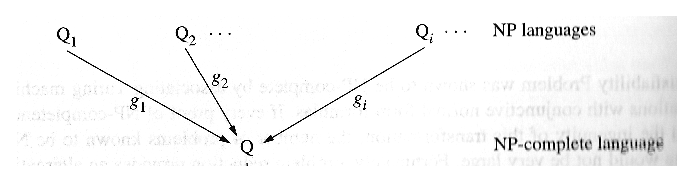
\includegraphics[height=20mm]{images/np-complete.eps}
\end{center}
\es

\bs{$NP$-Completeness}
\fframe{{\bf Theorem:} If $B$ is $NP$-complete and $B \in P$, then $P = NP$}

This theorem highlights the importance of $NP$-complete problems, should a deterministic polynomial time solutions be found to an $NP$-complete problem, then
the $NP$ complexity class will collapse into the $P$ complexity class.

\es

\bs{$NP$-Completeness}
\fframe{{\bf Theorem:}  If $B$ is $NP$-complete and $B \le_p C$ for $C \in NP$,
then $C$ is $NP$-complete.}

{\bf Proof:} Let $g_i$ be a polynomial time reduction from any language $A_i \in NP$ to $B$ and let $f$ be the polynomial time reduction from $B$ to $C$.  We know that $g_i$ has to exist for all languages $A_i \in NP$ since $B$ is $NP$-complete.  This gives us a polynomial time reduction $f \circ g_i$ from any language $A_i \in NP$ to $C$. $\Box$
\es

\end{document}
%%%%%%%%%%%%%%%%%%%%%%%%%%% end of template1.tex %%%%%%%%%%%%%%%%%%%%%%%%%%%%%%%%

